\section{Introduction}

\begin{frame}{Routing Problems}
	\note<1>[item]{
		Routing problems not only more prevalent and more complicated \begin{itemize}
			\item Navigation of vehicles or people between a predetermined set of points (like a set of customers)
			\item Some constraint or goal
			\item[$\Rightarrow$] Want optimal path or paths
		\end{itemize}
	}

	\note<1>[item] {
		Navigation in general \begin{itemize}
			\item Want to save time/fuel (shortest path)
			\item Want a beautiful trail to walk (highest quality path)
		\end{itemize}
	}
	\note<1>[item] {
		Online Shopping $\rightarrow$ shipping packages to customers \begin{itemize}
			\item Want to deliver the most packages in the smallest amount of time
		\end{itemize}
	}

	% Amazon

	\note<2->[item] {
		Example: Amazon \begin{itemize}
			\item $4.75$ billion shipped packages
			\item Need a way to manage this
		\end{itemize}
	}
	\note<2->[item] {
		Frequent Task: Optimize Routes in some respect\begin{itemize}
			\item Reduce fuel consumption/travel time
			\item Maximize profit gained
			\item How do I deliver the most goods while on a time budget?
			\item $\dots$ (you can think of a lot of things)
		\end{itemize}
	}

	\begin{columns}
		\begin{column}{0.48\textwidth}
			\begin{itemize}
				\item<1-> Routing problems are becoming more complicated \begin{itemize}
					\item<2-> Amazon with $\approx 4.75$ billion shipped packages \cite{placek_amazon_2022}
				\end{itemize}
			\end{itemize}
		\end{column}
		\begin{column}{0.48\textwidth}
			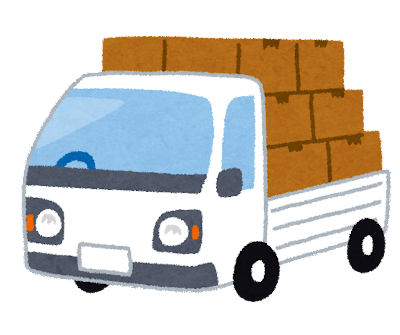
\includegraphics[width=0.7\textwidth]{res/truck_nimotsu.png}
		\end{column}
	\end{columns}

\end{frame}


\begin{frame}{Routing Problems}
	\note<1>[item] {Such problems are no stranger to computer science}
	\note<2>[item] {
		Most famous: Travelling Salesman Problem \begin{itemize}
			\item Graph
			\item Visit all nodes exactly once and return to the origin using the least distance
		\end{itemize}
	}
	\note<2>[item] {But there are also others}
	\note<3>[item] {
		Vehicle Routing Problem \begin{itemize}
			\item Generalization of the TSP
			\item Multiple vehicles starting at the origin
			\item[$\Rightarrow$] multiple routes minimizing the travel cost
		\end{itemize}
	}
	\note<4>[item] {
		\textbf{Orienteering Problem} \begin{itemize}
			\item No need to visit all nodes
			\item Nodes have scores/profit, edges have weights (omitted here for clarity)
			\item Time/distance limit
			\item Find a path (not necessarily cycle) with maximum profit that does not violate time/distance limit
			\item Now defined more accurately
		\end{itemize}
	}
	\begin{columns}
		\begin{column}{0.48\textwidth}
			\begin{itemize}
				\item<2-> Travelling Salesman Problem \cite{schrijver_history_2005}
				\item<3-> Vehicle Routing Problem \cite{dantzig_truck_1959}
				\item<4-> Orienteering Problem \cite{tsiligiridis_heuristic_1984}
			\end{itemize}
		\end{column}
		\begin{column}{0.48\textwidth}
			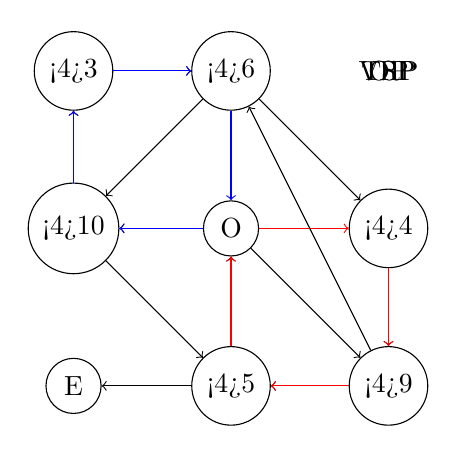
\begin{tikzpicture}[every node/.style={draw,shape=circle,minimum size=7mm}]
				\node (origin) at (0,0) {O};
				\node (1) at (-2,0) {\only<4>{10}};
				\node (2) at (-2,2) {\only<4>{3}};
				\node (3) at (0,2) {\only<4>{6}};
				\node (4) at (2,0) {\only<4>{4}};
				\node (5) at (0,-2) {\only<4>{5}};
				\node (6) at (2,-2) {\only<4>{9}};
				\node<4> (end) at (-2,-2) {E};

				% TSP 
				\node<2>[draw=none] (tsp) at (2,2) {TSP};
				\draw<2>[->] (origin) -- (1);
				\draw<2>[->] (1) -- (2);
				\draw<2>[->] (2) -- (3);
				\draw<2>[->] (3) -- (4);
				\draw<2>[->] (4) -- (6);
				\draw<2>[->] (6) -- (5);
				\draw<2>[->] (5) -- (origin);

				% VRP 
				\node<3>[draw=none] (vrp) at (2,2) {VRP};
				\draw<3>[->,blue] (origin) -- (1);
				\draw<3>[->,blue] (1) -- (2);
				\draw<3>[->,blue] (2) -- (3);
				\draw<3>[->,blue] (3) -- (origin);
				\draw<3>[->,red] (origin) -- (4);
				\draw<3>[->,red] (4) -- (6);
				\draw<3>[->,red] (6) -- (5);
				\draw<3>[->,red] (5) -- (origin);

				% OP
				\node<4>[draw=none] (op) at (2,2) {OP};
				\draw<4>[->] (origin) -- (6);
				\draw<4>[->] (6) -- (3);
				\draw<4>[->] (3) -- (1);
				\draw<4>[->] (1) -- (5);
				\draw<4>[->] (5) -- (end);

			\end{tikzpicture}
		\end{column}
	\end{columns}
\end{frame}
